\documentclass[11pt]{article}

\usepackage[margin=1in]{geometry}
\usepackage[T1]{fontenc}
\usepackage{mathptmx}
\usepackage{microtype}
\usepackage{graphicx}
\usepackage{booktabs}
\usepackage{amsmath}
\usepackage{xcolor}
\usepackage{tikz}
\usetikzlibrary{arrows.meta, positioning, fit}
\usepackage[font=small, labelfont=bf]{caption}
\usepackage{enumitem}
\usepackage{listings}
\usepackage[hidelinks]{hyperref}

\definecolor{codebg}{RGB}{246,247,249}
\definecolor{accent}{RGB}{37,99,235}
\lstset{
  basicstyle=\ttfamily\small,
  backgroundcolor=\color{codebg},
  frame=single, rulecolor=\color{codebg},
  breaklines=true, columns=fullflexible,
  xleftmargin=4pt, xrightmargin=4pt, aboveskip=8pt, belowskip=8pt
}
\setlist{itemsep=2pt, topsep=4pt}
\setlength{\emergencystretch}{3em}

\title{\textbf{DeepSentinel: Deepfake Face Detection with EfficientNet-B4,\\Grad-CAM Interpretability, and Cloud Deployment}}
\author{Aditya Chaudhary\\[2pt]
\small Purdue University\\
\small \href{https://github.com/adichaudhary/deepsentinel}{github.com/adichaudhary/deepsentinel}
\quad\textbullet\quad
\href{https://huggingface.co/spaces/adichaudhary/deepsentinel}{huggingface.co/spaces/adichaudhary/deepsentinel}}
\date{October 2026}

\begin{document}
\maketitle

\begin{abstract}
\noindent
DeepSentinel is an end-to-end system for detecting manipulated faces in images. An ImageNet-pretrained EfficientNet-B4 is fine-tuned as a binary classifier on face crops with identity-disjoint training, validation, and test splits, so reported results reflect performance on people the model has never seen. On a held-out, class-balanced test set of 4,000 images the model reaches \textbf{0.956 ROC AUC} and \textbf{88.8\% accuracy}. Grad-CAM is used to inspect which facial regions drive each prediction, and a masking ablation rules out a suspected shortcut. The trained model is served through a containerized FastAPI service with OpenCV face detection, deployed on AWS ECS Fargate, and exposed through an interactive Gradio demo on Hugging Face Spaces.
\end{abstract}

\section{Introduction}

Face manipulation tools have made it easy to produce convincing synthetic faces, which creates risk for identity verification, media integrity, and fraud prevention. Many deepfake detectors report strong numbers that do not hold up in practice because the same identities appear in both training and test data. In that setup a model can learn to recognize people rather than manipulation artifacts.

DeepSentinel addresses this in three ways. It evaluates only on identities that never appear during training. It uses Grad-CAM to make predictions inspectable and tests whether a suspicious activation pattern reflects a learned shortcut. And it carries the model through to production as a REST API on AWS and a public demo, using the same preprocessing at inference time as during evaluation.

\section{Data}

The model is trained on the Deepfake Identity Isolated Dataset \cite{dataset}, released under CC BY 4.0. It contains about 143K pre-cropped $260\times260$ face images labeled real or fake, split into training (99,910), validation (21,611), and test (21,316) sets with no identity overlap across splits.

For this work each split is subsampled to an equal number of real and fake images: 10,000 per class for training and 2,000 per class for validation and test. Balanced sampling keeps accuracy, precision, and recall directly interpretable. Labels are remapped so that $y=1$ denotes a manipulated face.

\section{Method}

\subsection{Model}

The classifier is EfficientNet-B4 \cite{efficientnet} initialized from ImageNet weights via \texttt{timm} \cite{timm}, with the classification head replaced by a single logit $z$. The predicted probability that a face is manipulated is $p = \sigma(z)$, and the model is trained with binary cross-entropy:
\begin{equation}
\mathcal{L} = -\big[\, y \log p + (1-y)\log(1-p) \,\big].
\end{equation}

\subsection{Preprocessing and Augmentation}

Each $260\times260$ crop is first center-cropped to $208\times208$ to remove image borders, then resized to $224\times224$ and normalized with ImageNet statistics. Training adds random resized crops (scale 0.8 to 1.0), horizontal flips, color jitter, Gaussian blur, and random erasing. Evaluation and deployment use only the deterministic center crop, resize, and normalization.

\subsection{Training}

The network is optimized with AdamW (learning rate $3\times10^{-4}$, weight decay $10^{-4}$) under a one-cycle learning rate schedule for 5 epochs with batch size 64. Training uses FP16 mixed precision with gradient scaling. The checkpoint with the highest validation ROC AUC is kept as the final model. Full optimizer, scheduler, and scaler state is checkpointed every epoch, so interrupted runs resume automatically. Training ran on a single NVIDIA GPU on Purdue's Scholar cluster, and metrics, configuration, and figures were logged to Weights \& Biases.

\section{Results}

\begin{table}[h]
\centering
\begin{tabular}{lcc}
\toprule
Metric & Validation & Test \\
\midrule
ROC AUC   & 0.954 & \textbf{0.956} \\
Accuracy  & 87.4\% & \textbf{88.8\%} \\
Precision & 89.5\% & \textbf{90.2\%} \\
Recall    & 84.8\% & \textbf{87.0\%} \\
F1        & 0.871 & \textbf{0.886} \\
\bottomrule
\end{tabular}
\caption{Classification performance at a threshold of 0.5. Validation figures are from the selected checkpoint (epoch 5). The test set contains 4,000 balanced images from identities not seen during training.}
\label{tab:results}
\end{table}

Table~\ref{tab:results} summarizes performance. Test results closely track validation results, which indicates the model generalizes to new identities rather than overfitting to the validation set used for checkpoint selection. Precision is somewhat higher than recall, so at the default threshold the model is slightly conservative about labeling a face as fake. Validation AUC rose steadily from 0.893 after the first epoch to 0.954 after the fifth.

\section{Interpretability and Robustness}

\begin{figure}[h]
\centering
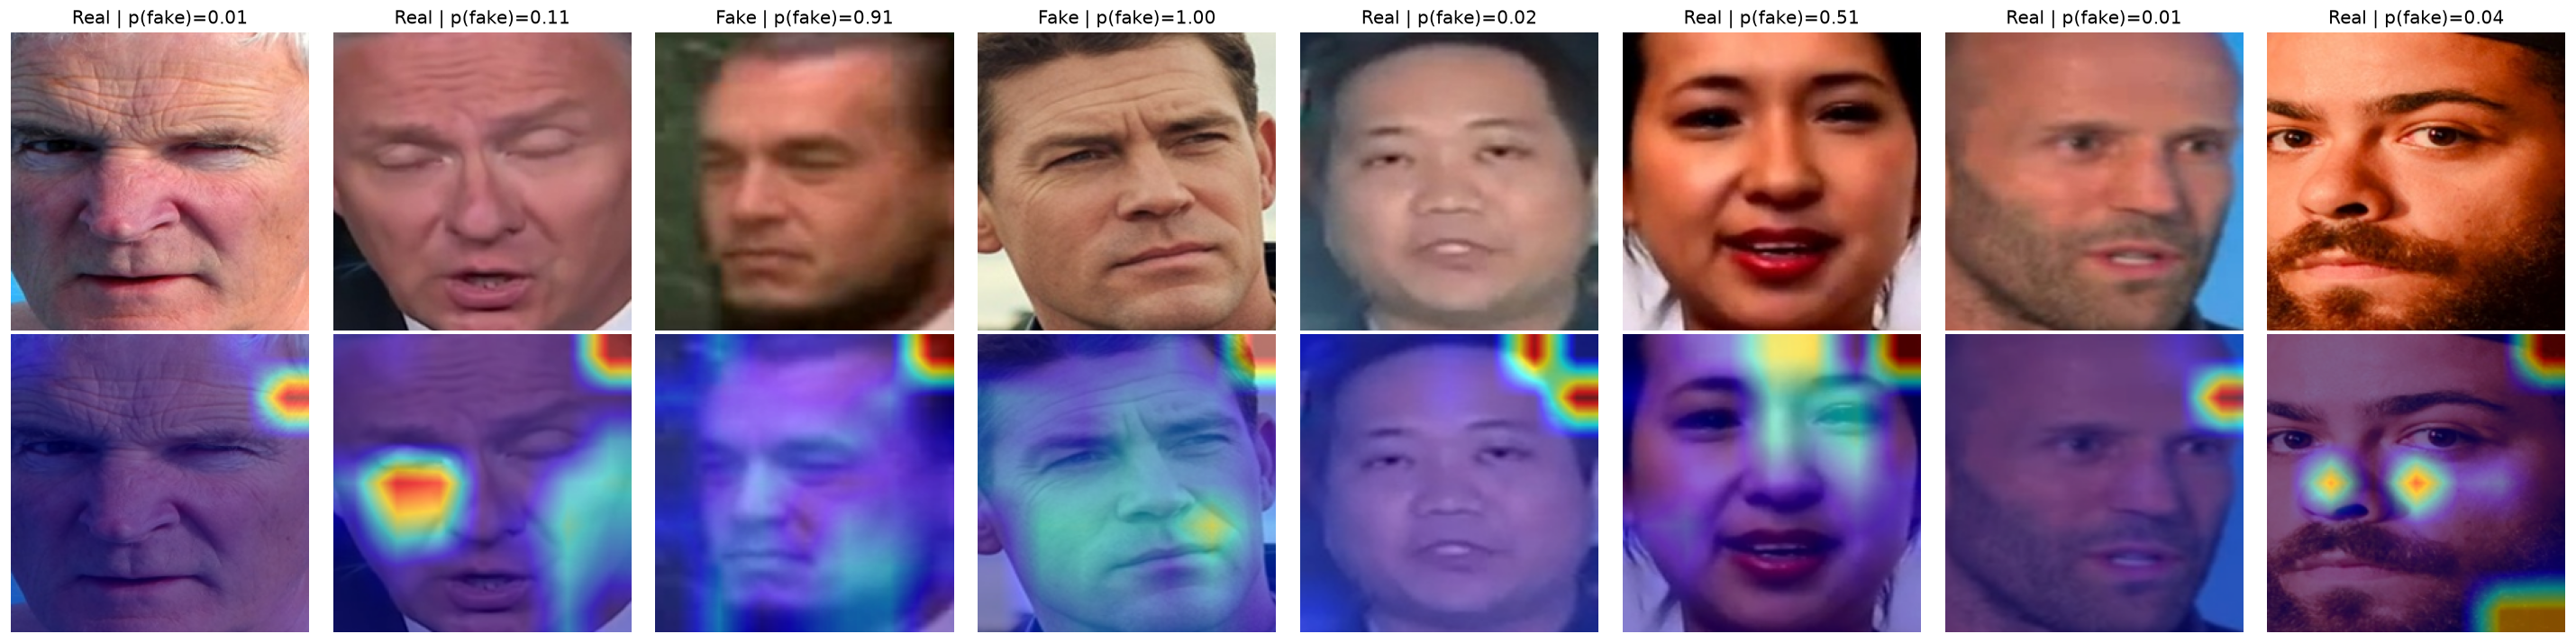
\includegraphics[width=\linewidth]{figures/gradcam.png}
\caption{Grad-CAM on held-out test images. Top row: inputs with ground-truth label and predicted probability of manipulation. Bottom row: class activation maps for the ``fake'' output.}
\label{fig:gradcam}
\end{figure}

Grad-CAM \cite{gradcam} computes class activation maps from the final convolutional layer. Figure~\ref{fig:gradcam} shows that for many faces the model attends to the eyes, nose, and cheeks, which are regions where face-swap blending artifacts commonly appear.

The maps also show a recurring hot spot in the top-right corner, including on real faces. This could mean the model learned a shortcut such as a watermark or encoding artifact in that region. Two checks were run to test this:
\begin{enumerate}
  \item \textbf{Border removal.} The model was retrained with a center crop that discards the outer border of every image. The corner activation persisted, even though the original corner pixels were no longer part of the input.
  \item \textbf{Masking ablation.} The top-right quarter of every test image was zeroed out at inference time. Test ROC AUC moved from 0.9557 to 0.9554.
\end{enumerate}
Because removing the region has no effect on performance, the corner activation is a boundary effect of the coarse $7\times7$ feature map that Grad-CAM upsamples, not information the classifier relies on.

\section{Deployment}

The trained model is packaged for production use and public demonstration. Figure~\ref{fig:arch} shows the overall architecture.

\begin{figure}[h]
\centering
\resizebox{\linewidth}{!}{%
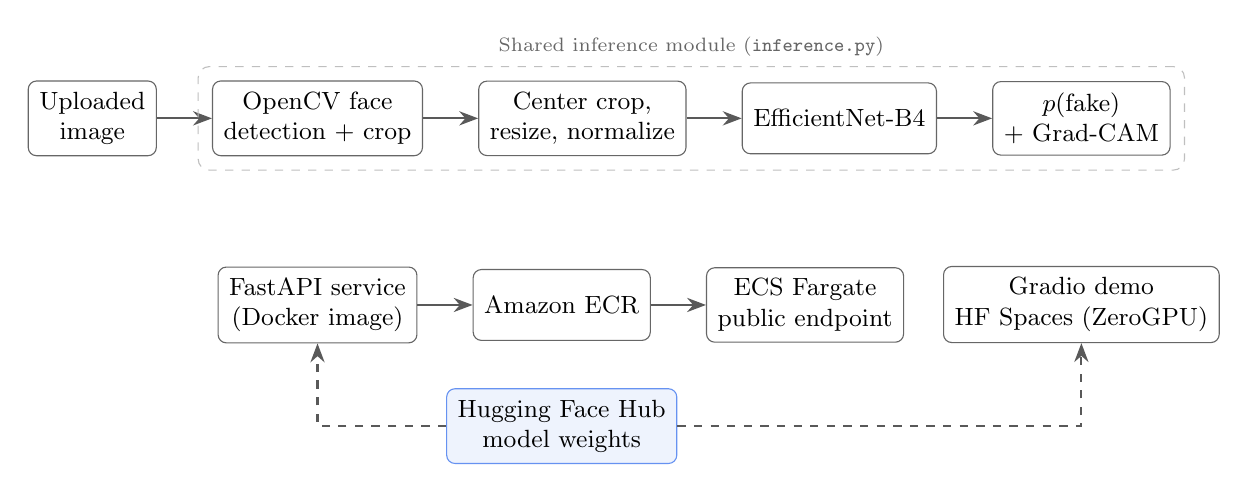
\begin{tikzpicture}[
  node distance=6mm and 7mm,
  box/.style={draw=black!60, rounded corners=3pt, align=center, font=\small, minimum height=9mm, inner sep=4pt, fill=white},
  hub/.style={box, fill=accent!8, draw=accent!70},
  arr/.style={-{Stealth[length=2.4mm]}, thick, black!65}
]
\node[box] (img) {Uploaded\\image};
\node[box, right=of img] (det) {OpenCV face\\detection + crop};
\node[box, right=of det] (pre) {Center crop,\\resize, normalize};
\node[box, right=of pre] (model) {EfficientNet-B4};
\node[box, right=of model] (out) {$p(\text{fake})$\\+ Grad-CAM};
\draw[arr] (img) -- (det);
\draw[arr] (det) -- (pre);
\draw[arr] (pre) -- (model);
\draw[arr] (model) -- (out);

\node[box, below=14mm of det] (api) {FastAPI service\\(Docker image)};
\node[box, right=of api] (ecr) {Amazon ECR};
\node[box, right=of ecr] (ecs) {ECS Fargate\\public endpoint};
\node[box, below=14mm of out] (space) {Gradio demo\\HF Spaces (ZeroGPU)};
\node[hub, below=6mm of ecr] (hub) {Hugging Face Hub\\model weights};
\draw[arr] (api) -- (ecr);
\draw[arr] (ecr) -- (ecs);
\draw[arr, dashed] (hub.west) -| (api.south);
\draw[arr, dashed] (hub.east) -| (space.south);

\node[draw=black!25, dashed, rounded corners=4pt, fit=(det)(pre)(model)(out), inner sep=5pt,
      label={[font=\scriptsize, text=black!60]above:Shared inference module (\texttt{inference.py})}] {};
\end{tikzpicture}%
}
\caption{Inference pipeline (top) and serving architecture (bottom). Both serving paths use the same inference module and pull weights from the Hugging Face Hub.}
\label{fig:arch}
\end{figure}

\subsection{Inference Pipeline}

Training data consists of tight face crops, but real uploads are arbitrary photos. The inference module bridges that gap so the model sees inputs that match its training distribution:
\begin{enumerate}
  \item \textbf{Face detection.} OpenCV's frontal-face Haar cascade \cite{opencv} locates faces. The largest face is selected and cropped as a square with a 25\% margin. If no face is found, the module falls back to a centered square crop and reports that in the response.
  \item \textbf{Preprocessing.} The crop is resized to $260\times260$ to match the dataset, then passed through the exact evaluation transform from training (center crop to 208, resize to 224, ImageNet normalization).
  \item \textbf{Prediction and explanation.} The model returns $p(\text{fake})$ and a label at a 0.5 threshold. Grad-CAM optionally produces an overlay on the preprocessed face.
\end{enumerate}
The same module is used by both the REST API and the Gradio demo, so the two cannot drift apart.

\subsection{Model Hosting}

The trained weights (\texttt{deepsentinel\_effb4.pt}) are published to the Hugging Face Hub at \texttt{adichaudhary/deepsentinel}. Both serving paths download weights from this single source, so updating the model requires only a new upload and a redeploy.

\subsection{REST API}

The API is built with FastAPI and exposes three endpoints:

\begin{table}[h]
\centering
\begin{tabular}{ll}
\toprule
Endpoint & Description \\
\midrule
\texttt{GET /health} & Liveness check and model load status \\
\texttt{POST /predict} & Multipart image upload. Returns \texttt{label}, \texttt{p\_fake}, face box, \\
                       & and an optional base64 Grad-CAM PNG (\texttt{?heatmap=true}) \\
\texttt{GET /docs} & Interactive OpenAPI documentation \\
\bottomrule
\end{tabular}
\end{table}

\noindent The model loads once at startup through FastAPI's lifespan handler, so requests do not pay model-loading cost. Uploads are capped at 10\,MB, and invalid files return HTTP 400. Responses are validated with Pydantic models. The following request was sent to the live ECS deployment with a held-out manipulated face from the test set:

\begin{lstlisting}
curl -F "file=@sample_fake.png" "http://<ecs-endpoint>:8000/predict"

{"label": "fake", "p_fake": 0.9992, "face_detected": true,
 "face_box": [0, 0, 331, 331], "heatmap_png_base64": null}
\end{lstlisting}
Passing \texttt{?heatmap=true} adds the Grad-CAM overlay as a base64-encoded PNG.

\subsection{Containerization}

The service is packaged with Docker on a \texttt{python:3.12-slim} base. Design choices for the image:
\begin{itemize}
  \item \textbf{CPU-only PyTorch} wheels keep the image far smaller than a CUDA build, and EfficientNet-B4 inference on a single image is fast enough on CPU for this workload.
  \item \textbf{Weights are baked in at build time} from the Hugging Face Hub, so containers start without a network fetch and every image is tied to a fixed model version.
  \item \textbf{Hardening:} the container runs as a non-root user, a \texttt{.dockerignore} allowlist keeps everything except the application code out of the build context, and a Docker \texttt{HEALTHCHECK} polls \texttt{/health}.
\end{itemize}

\subsection{AWS ECS Deployment}

The container runs on AWS ECS with the Fargate launch type, which removes the need to manage servers. A single script, \texttt{deploy/deploy.sh}, handles the full deployment and is safe to rerun:
\begin{enumerate}
  \item Creates an Amazon ECR repository if needed, then builds the image for \texttt{linux/amd64} and pushes it.
  \item Creates the ECS task execution role with the \texttt{AmazonECSTaskExecutionRolePolicy} if it does not exist.
  \item Registers a task definition (1 vCPU, 3\,GB memory) with a container health check and CloudWatch Logs through the \texttt{awslogs} driver.
  \item Creates the ECS cluster and a security group that allows inbound traffic on port 8000 in the default VPC.
  \item Creates the Fargate service with a public IP, or forces a new deployment if the service already exists.
  \item Waits for the service to stabilize and prints the public endpoint.
\end{enumerate}
A companion script, \texttt{deploy/teardown.sh}, scales the service to zero and removes the service and cluster to stop billing while keeping the image in ECR for fast redeploys.

\subsection{Interactive Demo}

A Gradio application on Hugging Face Spaces gives anyone a browser-based way to try the model. Users upload a photo and receive class probabilities and a Grad-CAM overlay. The Space runs on ZeroGPU hardware, which attaches a GPU only while a request is being processed. Figure~\ref{fig:demo} shows the deployed demo on two held-out test images.

\begin{figure}[h]
\centering
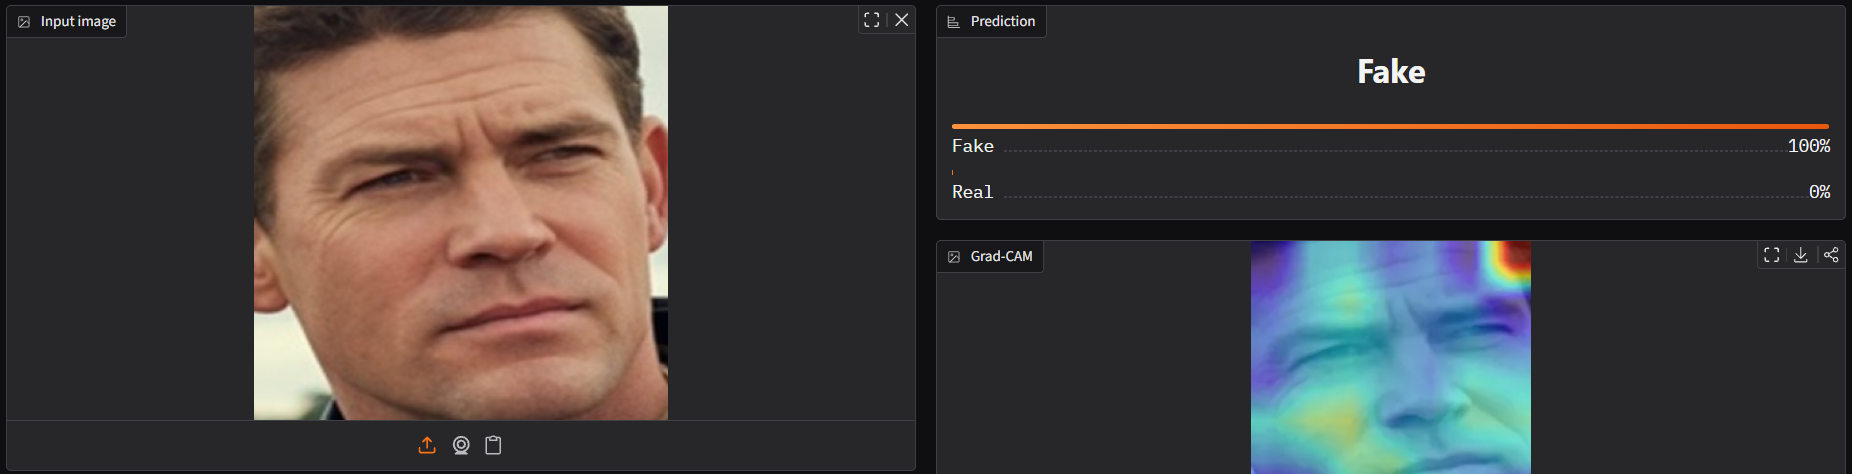
\includegraphics[width=\linewidth]{figures/demo_fake.png}\\[6pt]
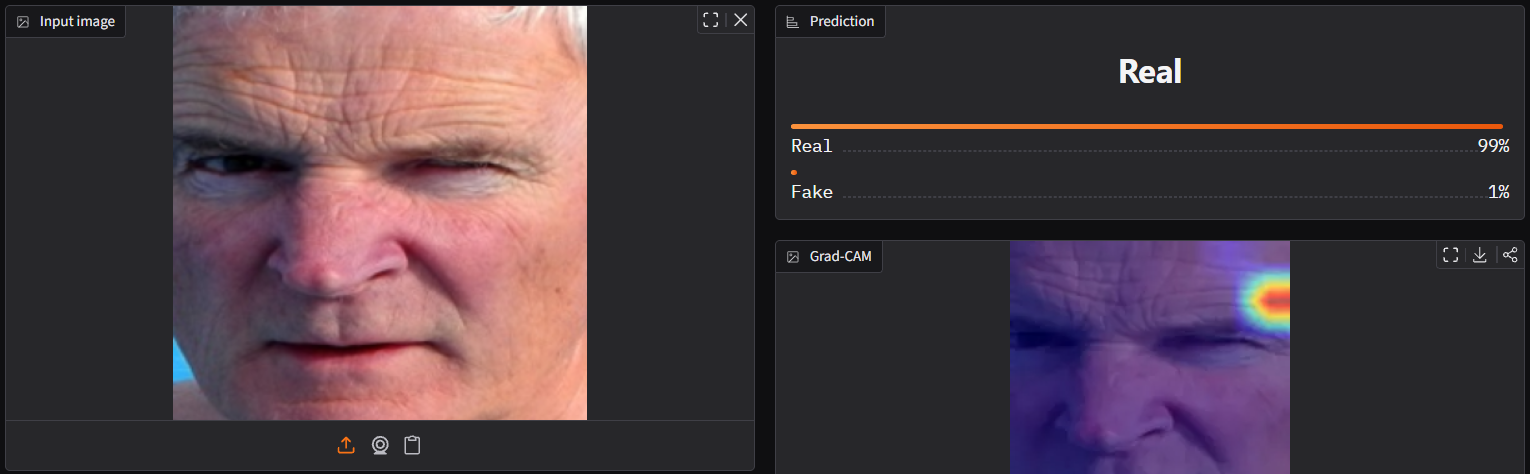
\includegraphics[width=\linewidth]{figures/demo_real.png}
\caption{The live Hugging Face Spaces demo on held-out test images. Top: a manipulated face classified as fake with 100\% confidence. Bottom: a real face classified as real with 99\% confidence. Each result includes a Grad-CAM overlay.}
\label{fig:demo}
\end{figure}

\section{Limitations and Future Work}

\begin{itemize}
  \item \textbf{Single dataset.} Results come from one dataset. Cross-dataset evaluation on benchmarks such as FaceForensics++ \cite{ffpp} and Celeb-DF \cite{celebdf} would test generalization to unseen manipulation methods.
  \item \textbf{Still images only.} The model scores individual frames. Video detection could aggregate frame scores or use temporal models to catch flicker and inconsistencies across frames.
  \item \textbf{Training subset.} Only 20K of the roughly 100K available training images were used. Training on the full split and at the native B4 resolution of $380\times380$ is likely to improve results.
  \item \textbf{Face detector.} The Haar cascade is fast but misses profile and heavily occluded faces. A learned detector would improve robustness in production.
  \item \textbf{Calibration.} The 0.5 threshold is not tuned. Calibrating probabilities and choosing a threshold for a target false positive rate would suit real moderation workflows better.
\end{itemize}

\section{Conclusion}

DeepSentinel shows a complete path from research to deployment for deepfake detection. A fine-tuned EfficientNet-B4 reaches 0.956 ROC AUC on identities it has never seen. Grad-CAM analysis, paired with border removal and a masking ablation, confirms that the model does not rely on a spurious corner artifact. The model is served through a containerized FastAPI service on AWS ECS Fargate and a public Gradio demo, both sharing one inference module and one source of model weights.

\begin{thebibliography}{9}\small
\bibitem{dataset} ThinothW. \textit{Deepfake Identity Isolated Dataset (PreP)}. Hugging Face. \url{https://huggingface.co/datasets/ThinothW/Deepfake-Identity-Isolated-Dataset-PreP}
\bibitem{efficientnet} M. Tan and Q. V. Le. EfficientNet: Rethinking Model Scaling for Convolutional Neural Networks. In \textit{ICML}, 2019.
\bibitem{gradcam} R. R. Selvaraju, M. Cogswell, A. Das, R. Vedantam, D. Parikh, and D. Batra. Grad-CAM: Visual Explanations from Deep Networks via Gradient-based Localization. In \textit{ICCV}, 2017.
\bibitem{timm} R. Wightman. PyTorch Image Models. \url{https://github.com/huggingface/pytorch-image-models}, 2019.
\bibitem{opencv} P. Viola and M. Jones. Rapid Object Detection using a Boosted Cascade of Simple Features. In \textit{CVPR}, 2001.
\bibitem{ffpp} A. R\"ossler, D. Cozzolino, L. Verdoliva, C. Riess, J. Thies, and M. Nie{\ss}ner. FaceForensics++: Learning to Detect Manipulated Facial Images. In \textit{ICCV}, 2019.
\bibitem{celebdf} Y. Li, X. Yang, P. Sun, H. Qi, and S. Lyu. Celeb-DF: A Large-scale Challenging Dataset for DeepFake Forensics. In \textit{CVPR}, 2020.
\end{thebibliography}

\end{document}
